\tocless\subsection{Objective}
In our previous sliding window-oriented experiments, we had only used a
single image. In order to see whether this image had biases unknown
to us, another fruit bowl image had to be tested. This image was selected as
fruit took up a larger portion of the image as seen in Figure \ref{fig:newFruit}.

\begin{figure}[h]
\centering
    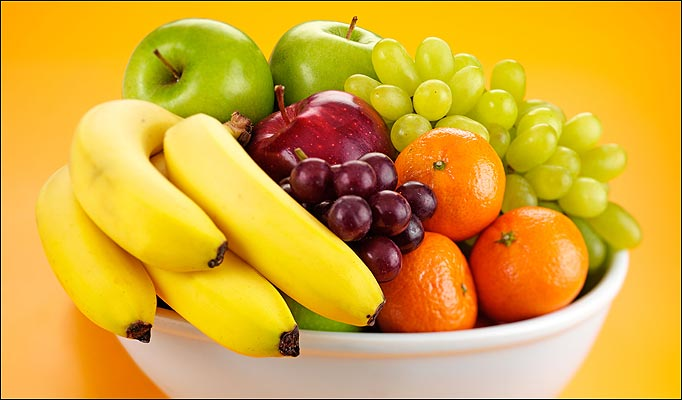
\includegraphics[scale=0.4]{fruitbowl2}
    \caption{Alternative Bowl of fruit}
    \label{fig:newFruit}
\end{figure}

\begin{table}[]
    \centering
    \caption{Comparison of fruit bowl images}
    \label{newFruitTable}
    \begin{tabular}{|l|l|l|l|p{1.25cm}|p{1.25cm}|p{2cm}|}
    \hline
        \textbf{Food type} & \textbf{Grid} & \textbf{Row} & \textbf{Column} & \textbf{New Grid} & \textbf{New Row} & \textbf{New Column} \\ \hline
        Apple     & 5    & 1   & 3      & 4        & 1       & 0          \\ \hline
        Banana    & 1    & 0   & 1      & 5        & 0       & 5          \\ \hline
        Grape     & 4    & 0   & 0      & 2        & 1       & 0          \\ \hline
        Orange    & 5    & 0   & 0      & 0        & 0       & 0          \\ \hline
        Other     & 0    & 3   & 1      & 1        & 2       & 1         \\ \hline
    \end{tabular}
\end{table}

\tocless\subsection{Results}
\tocless\subsubsection{Grid}
The performance of this experiment was slightly worse than with the previously
used image. When the grid based sliding window was executed on Figure
\ref{fig:newFruit}, fourteen out of fifteen predictions had an expected value.
Out of the fourteen predictions orange was not predicted to top-1 accuracy at
all. This can be seen, in comparison to previously used image, in Table
\ref{newFruitTable}.

\tocless\subsubsection{Row}
In the column based window for the new fruit image, the results were not very
successful as has been the trend for most row based classification. Two out of
four predictions had an expected value at top-1 accuracy.

\tocless\subsubsection{Column}
The column based approach had a similar result to its counterpart in that only
one of its predictions was unexpected. Although, due  to the size of the new
image, another column was created and thus has a better overall accuracy.

\tocless\subsection{Analysis}
A possible reason that an orange was not classified in any of these images is
because in Figure \ref{fig:newFruit}, a more mandarin food is displayed.
